\documentclass[letterpaper]{article}
\usepackage[margin=1in]{geometry}
\usepackage[utf8]{inputenc}
\usepackage{textcomp}
\usepackage{amssymb}
\usepackage{natbib}
\usepackage{graphicx}
\usepackage{gensymb}
\usepackage{amsthm, amsmath, mathtools}
\usepackage[dvipsnames]{xcolor}
\usepackage{enumerate}
\usepackage{mdframed}
\usepackage[most]{tcolorbox}
\usepackage{csquotes}
% https://tex.stackexchange.com/questions/13506/how-to-continue-the-framed-text-box-on-multiple-pages

\tcbuselibrary{theorems}

\newcommand{\R}{\mathbb{R}}
\newcommand{\Z}{\mathbb{Z}}
\newcommand{\N}{\mathbb{N}}
\newcommand{\Q}{\mathbb{Q}}
\newcommand{\C}{\mathbb{C}}
\newcommand{\code}[1]{\texttt{#1}}
\newcommand{\mdiamond}{$\diamondsuit$}
\newcommand{\PowerSet}{\mathcal{P}}
\newcommand{\Mod}[1]{\ (\mathrm{mod}\ #1)}
\DeclareMathOperator{\lcm}{lcm}

%\newtheorem*{theorem}{Theorem}
%\newtheorem*{definition}{Definition}
%\newtheorem*{corollary}{Corollary}
%\newtheorem*{lemma}{Lemma}
\newtheorem*{proposition}{Proposition}


\newtcbtheorem[number within=section]{theorem}{Theorem}
{colback=green!5,colframe=green!35!black,fonttitle=\bfseries}{th}

\newtcbtheorem[number within=section]{definition}{Definition}
{colback=blue!5,colframe=blue!35!black,fonttitle=\bfseries}{def}

\newtcbtheorem[number within=section]{corollary}{Corollary}
{colback=yellow!5,colframe=yellow!35!black,fonttitle=\bfseries}{cor}

\newtcbtheorem[number within=section]{lemma}{Lemma}
{colback=red!5,colframe=red!35!black,fonttitle=\bfseries}{lem}

\newtcbtheorem[number within=section]{example}{Example}
{colback=white!5,colframe=white!35!black,fonttitle=\bfseries}{def}

\newtcbtheorem[number within=section]{note}{Important Note}{
        enhanced,
        sharp corners,
        attach boxed title to top left={
            xshift=-1mm,
            yshift=-5mm,
            yshifttext=-1mm
        },
        top=1.5em,
        colback=white,
        colframe=black,
        fonttitle=\bfseries,
        boxed title style={
            sharp corners,
            size=small,
            colback=red!75!black,
            colframe=red!75!black,
        } 
    }{impnote}
\usepackage[utf8]{inputenc}
\usepackage[english]{babel}
\usepackage{fancyhdr}
\usepackage[hidelinks]{hyperref}

\pagestyle{fancy}
\fancyhf{}
\rhead{CSE 105}
\chead{Monday, January 24, 2022}
\lhead{Lecture 6}
\rfoot{\thepage}

\setlength{\parindent}{0pt}

\begin{document}

\section{Regular Expressions (1.3)}
We can use \textbf{regular expressions} (RegExp) to describe a language. An example of a regular expression is: 
\[(\code{0} \cup \code{1}) \code{0}^*\]
To give a comparison, consider the arithmetic expression:
\[(5 + 4) \times 2\]
In an arithmetic expression, the value is a number; in our case above, we would get 18. In a regular expression, the value is a \textbf{language}; in our case above, we can break the expression into multiple parts: 
\begin{itemize}
    \item $\code{0} \cup \code{1}$: This is the same thing as saying $\{\code{0}\} \cup \{\code{1}\}$, so this segment is saying that its language is $\{\code{0}, \code{1}\}$.
    \item $\code{0}^*$: This is the same thing as saying $\{\code{0}\}^*$, so its value is the language consisting of all strings containing any numbers of \code{0}s.
\end{itemize}
Putting it together, this regular expression recognizes any string which starts with \code{0} or \code{1} and ends with some number of \code{0}s. Just like how the multiplication sign $\times$ is often implicitly written (that is, we can write $2(5 + 4)$ instead of $2 \times (5 + 4)$), the concatenation sign $\circ$ is also implicitly written. That is, $(\code{0} \cup \code{1}) \code{0}^*$ is the shorthand for $(\code{0} \cup \code{1}) \circ \code{0}^*$. 

\subsection{Formal Definition of a Regular Expression}
\begin{definition}{Regular Expression}{}
    We say that $R$ is a \textbf{regular expression} if $R$ is: 
    \begin{enumerate}
        \item $a$ for some $a$ in the alphabet $\Sigma$,
        \item $\epsilon$,
        \item $\emptyset$,
        \item $(R_1 \cup R_2)$, where $R_1$ and $R_2$ are regular expressions,
        \item $(R_1 \circ R_2)$, where $R_1$ and $R_2$ are regular expressions,
        \item $(R_1^*)$, where $R_1$ is a regular expressions,
    \end{enumerate}
    In items 1 and 2, the regular expressions $a$ and $\epsilon$ represent the languages $\{a\}$ and $\{\epsilon\}$, respectively. In item 3, the regular expression $\emptyset$ represents the empty language. In items 4, 5, and 6, the expressions represent the languages obtained by taking the union or concatenation of the languages $R_1$ and $R_2$, or the star of the language $R_1$, respectively. 
\end{definition}
\textbf{Remarks:}
\begin{itemize}
    \item Remember, $\epsilon$ and $\emptyset$ are not the same. $\epsilon$ is the same thing as $\{\epsilon\}$, i.e. the language containing only the empty string; however, $\emptyset$ represents the language that doesn't contain anything. 
    \item In regular expressions, there is the notion of operator precedence. In our case, the star operation is done first, followed by concatenation, and finally union \emph{unless} parentheses change the usual order.
    \item We may omit the $\circ$ notation for concatenation. For example, $R_1 R_2$ is the same thing as $R_1 \circ R_2$.  
\end{itemize}
Additionally, we define some more notation.
\begin{itemize}
    \item Let $R^+$ be shorthand for $RR^*$. In other words, while $R^*$ has all strings that are 0 or more concatenations of strings from $R$, the language $R^+$ has all strings that are \textbf{1} or more concatenations of strings from $R$. So, really, $R^+ \cup \epsilon = R^*$. 
    \item We let $R^k$ be shorthand for the concatenation of $k$ $R$'s with each other. 
\end{itemize}
Finally, when we want to distinguish between a regular language $R$ and the language it described, we write $L(R)$ to be the language of $R$. 

\subsubsection{Example: Regular Languages}
Suppose $\epsilon = \{\code{0}, \code{1}\}$. Then, some examples of regular expressions are: 
\begin{center}
    \begin{tabular}{p{1.2in}|p{1.8in}|p{3in}}
        \textbf{RegExp} & \textbf{Examples} & \textbf{Formal Description} \\ 
        \hline 
        $\code{0}^* \code{10}^*$ & \code{1}, \code{01}, \code{0100} & $\{w \mid w \text{ contains a single } \code{1}\}$ \\ 
        \hline 
        $\Sigma^{*}\code{1}\Sigma^{*}$ & \code{1}, \code{00101101} & $\{w \mid w \text{ has at least one } \code{1}\}$ \\ 
        \hline 
        $\Sigma^{*}\code{001}\code{*}$ & \code{001}, \code{0100101} & $\{w \mid w \text{ contains the string } \code{001} \text{ as a substring}\}$ \\ 
        \hline 
        $\code{1}^* (\code{01}^+)^*$ & \code{1010110111}, \code{1110101} & $\{w \mid \text{every } \code{0} \text{ in } w \text{ is followed by at least one } \code{1}\}$ \\ 
        \hline 
        $\underbrace{(\Sigma\Sigma \dots \Sigma\Sigma)^{*}}_{n \text{ times}}$ & & $\{w \mid \text{the length of } w \text{ is a multiple of } n\}$ \\ 
        \hline 
        $\code{01} \cup \code{10}$ & \code{10}, \code{01} & $\{\code{01}, \code{10}\}$ \\ 
        \hline 
        $\code{0}\Sigma^* \code{0} \cup \code{1} \Sigma^* \code{1} \cup \code{0} \cup \code{1}$ & \code{00}, \code{11}, \code{10101}, \code{0}, \code{1} & $\{w \mid w \text{ starts and ends with the same symbol}\}$ \\ 
        \hline 
        $(\code{0} \cup \epsilon)\code{1}^*$ & \code{11111}, \code{01}, \code{0111} & $\code{01}^* \cup 1^*$ \\ 
        \hline 
        $(\code{0} \cup \epsilon)(\code{1} \cup \epsilon)$ & \code{01}, \code{1}, \code{0}, $\epsilon$ & $\{\epsilon, \code{0}, \code{1}, \code{01}\}$ \\ 
        \hline 
        $\code{1}^* \emptyset$ & & $\emptyset$ \\ 
        \hline 
        $\emptyset^*$ & $\epsilon$ & $\{\epsilon\}$
    \end{tabular}
\end{center}
\textbf{Remarks:}
\begin{itemize}
    \item Concatenating the empty set to any set yields the empty set. 
    \item The star operation on the empty set produces the set containing only the empty string. 
\end{itemize}

\subsection{Identities}
Let $R$ be any regular expression. The following identities hold:
\begin{enumerate}
    \item $R \cup \emptyset = R$. Adding the empty language to any other language will not change it. 
    \item $R \circ \epsilon = R$. Joining the empty string to any string will not change it. 
\end{enumerate}
As a warning, the following do not necessarily hold: 
\begin{enumerate}
    \item $R \cup \epsilon = R$. If $R = \code{0}$, then $L(R) = \{\code{0}\}$ but $L(R \cup \epsilon) = \{\code{0}, \epsilon\}$
    \item $R \circ \emptyset = R$. If $R = \code{0}$, then $L(R) = \{\code{0}\}$ but $L(R \circ \emptyset) = \emptyset$. 
\end{enumerate}

\subsection{Practical Applications of RegExp}
Regular expressions have practical applications. One example is in the world of compilers for programming languages. In particular, elemental objects in a programming language, called \textbf{tokens}, such as variable names and constants, can be described with regular expression. Consider the following regular expression:
\[(\code{+} \cup \code{-} \cup \epsilon)(D^+ \cup D^+ \code{.} D^* \cup D^* \code{.} D^+)\]
Where $D = \{\code{0}, \code{1}, \code{2}, \dots, \code{8}, \code{9}\}$. This regular expression describes a numerical constant which may include a fractional part and/or a sign. For example, the following strings are valid: 
\begin{itemize}
    \item \code{3.1415926}
    \item \code{+2.}
    \item \code{-.15}
\end{itemize}
After we can describe the syntax of a programming language with a regular expression in terms of its tokens, we can generate a \textbf{lexical analyzer} which processes it. 

\subsection{Generalized Nondeterministic Finite Automaton}
We now introduce a new type of finite automaton called a \textbf{generalized nondeterministic finite automaton}, also known as a GNFA. First, we briefly introduce what a GNFA is:
\begin{itemize}
    \item GNFAs are simply nondeterministic finite automata wherein the transition arrows may have any \emph{regular expressions} as labels, instead of only members of the alphabet or $\epsilon$. 
    \item The GNFA reads \emph{blocks of symbols} form the input, not necessarily just one symbol at a time.
    \item The GNFA moves along a transition arrow connecting two states by reading a block of symbols from the input, which themselves constittue a string described by the regular expression on that arrow. 
    \item GNFAs are nondeterministic, so there may be several different ways to process the same input string.
\end{itemize}
\begin{center}
    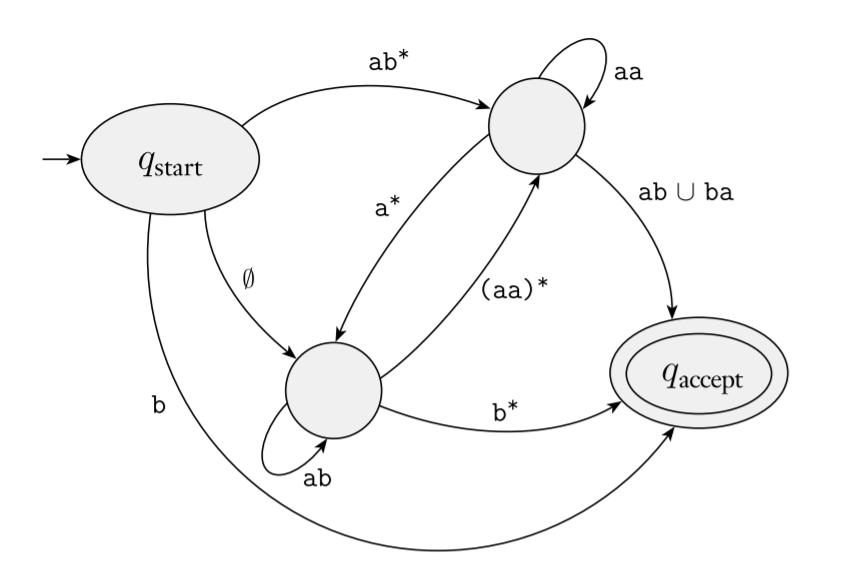
\includegraphics[scale=0.4]{../assets/gnfa_ex_1.png}

    \textbf{Figure:} A generalized nondeterministic finite automaton.
\end{center}
We always require GNFAs to have a special form that meets the following conditions: 
\begin{enumerate}
    \item The \underline{start state} has transition arrows going to every other state but no arrows coming in from any other state. 
    \item There is only a single accept state, and it has arrows coming in from every other state but no arrows going to any other state. Additionally, the start state cannot be the accept state. 
    \item For all other states except the start/accept states, one arrow goes from every state to every other state and also from each state to itself. 
\end{enumerate}

\subsubsection{DFA to GNFA}
To convert a DFA to a GNFA, we do the following: 
\begin{itemize}
    \item We can add a new start state with a $\epsilon$ arrow to the old start state and a new accept state with $\epsilon$ from the old accept states. 
    \item If any arrows have multiple labels, or if there are multiple arrows going between the same two states in the same direction, replace each with a single arrow whose label is the union of the previous labels.
    \item Finally, add arrows labeled $\emptyset$ between states that have no arrows. 
\end{itemize}

\subsubsection{GNFA to Regular Expression}
We now need to convert a GNFA to a regular expression. Say that a GNFA has $k$ states. Then, because a GNFA must have a start and an accept state and they must be different from each other, we know that $k \geq 2$. If $k > 2$, we construct an equivalent GNFA with $k - 1$ states. We continue to do this until the GNFA is reduced to two states. If $k = 2$, then the GNFA has a single arrow that goes from the start state to the accept state. The label of this arrow would then be the \emph{equivalent regular expression}.

\bigskip 

The most important step in this process is constructing an equivalent GNFA with one fewer state when $k > 2$. How can we do this? Well: 
\begin{itemize}
    \item Select a state that isn't the start or accept state, rip that state out of the machine, and then repairing what is left of the machine so the same language is still recognized. Call this state $q_{\text{rip}}$.
    \item After removing $q_{\text{rip}}$, we need to repair the machine by altering the regular expressions that label each of the remaining arrows. We use these new labels because they add back the lost computations (from ripping $q_{\text{rip}}$). 
\end{itemize}
Consider the following GNFA: 
\begin{center}
    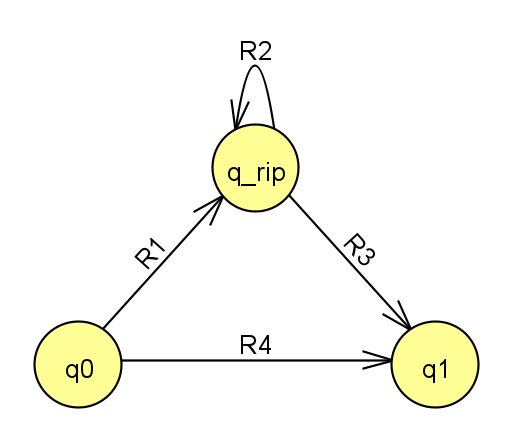
\includegraphics[scale=0.4]{../assets/gnfa_before.png}
\end{center}
If we remove $q_{\text{rip}}$, we get the following GNFA: 
\begin{center}
    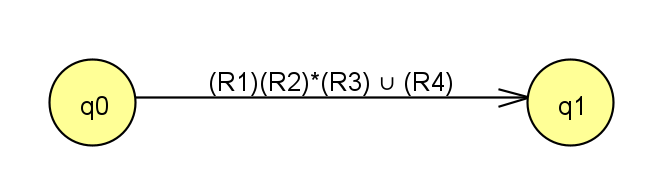
\includegraphics[scale=0.4]{../assets/gnfa_after.png}
\end{center}
Essentially, in the old machine, if: 
\begin{enumerate}
    \item $q_0$ goes to $q_{\text{rip}}$ with an arrow labeled $R_1$, and 
    \item $q_{\text{rip}}$ goes to itself with an arrow labeled $R_2$, and 
    \item $q_{\text{rip}}$ goes to $q_1$ with an arrow labeld $R_3$, and 
    \item $q_0$ goes to $q_1$ with an arrow labeled $R_4$
\end{enumerate}
Then, in the new revised machine, the arrow from $q_0$ to $q_1$ gets the label 
\[(R_1)(R_2)^* (R_3) \cup (R_4)\]
We can make this change for each arrow going from any state $q_0$ to any state $q_1$, including when $q_0 = q_1$. 

\subsubsection{Formal Definition}
The formal definition of a GNFA is: 
\begin{definition}{Generalized Nondeterministic Finite Automaton}{}
    A \textbf{generalized nondeterministic finite automaton} is a 5-tuple $(Q, \Sigma, \delta, q_{\text{start}}, q_{\text{accept}})$ where 
    \begin{enumerate}
        \item $Q$ is the finite set of tuples. 
        \item $\Sigma$ is the input alphabet. 
        \item $\delta: (Q \setminus \{q_{\text{accept}}\}) \times (Q \setminus \{q_{\text{start}}\}) \mapsto \mathcal{R}$ is the transition function. 
        \item $q_{\text{start}}$ is the start state. 
        \item $q_{\text{accept}}$ is the accept state. 
    \end{enumerate}
\end{definition}
\textbf{Remarks:}
\begin{itemize}
    \item Here, $\mathcal{R}$ is the collection of all regular expressions over the alphabet $\Sigma$. 
    \item If $\delta(q_i, q_j) = R$, then the arrow from state $q_i$ to state $q_j$ has the regular expression $R$ as its label. 
\end{itemize}

\subsubsection{Convert Algorithm}
Suppose $G$ is an GNFA. Then, the $\code{CONVERT}(G)$ algorithm takes a GNFA and returns an equivalent regular expression. The algorithm works like so (Page 73): 
\begin{mdframed}[]
    $\code{CONVERT}(G)$
    \begin{enumerate}
        \item Let $k$ be the number of states of $G$. 
        \item If $k = 2$, then $G$ must consist of a start state, an accept state, and a single arrow connecting them and labeled with a regular expression $R$. So, return $R$. 
        \item Otherwise, $k > 2$ so we select any state $q_{\text{rip}} \in Q$ different from $q_{\text{start}}$ and $q_{\text{accept}}$. Let $G'$ be the GNFA $(Q', \Sigma, \delta', q_{\text{start}}, q_{\text{accept}})$ where $Q' = Q \setminus \{q_{\text{rip}}\}$ and, for any $q_i \in G' \setminus \{q_{\text{accept}}\}$ and $q_j \in Q' \setminus \{q_{\text{start}}\}$, let
        \[\delta'(q_i, q_j) = (R_1)(R_2)^* (R_3) \cup (R_4)\]
        Where $R_1 = \delta(q_i, q_{\text{rip}})$, $R_2 = \delta(q_{\text{rip}}, q_{\text{rip}})$, $R_3 = (q_{\text{rip}}, q_j)$, and $R_4 = \delta(q_i, q_j)$. 
        \item Compute $\code{CONVERT}(G')$. 
    \end{enumerate}
\end{mdframed}

\subsubsection{Example 1: DFA to Regular Expression}
Suppose we wanted to convert the following DFA to a regular expression:
\begin{center}
    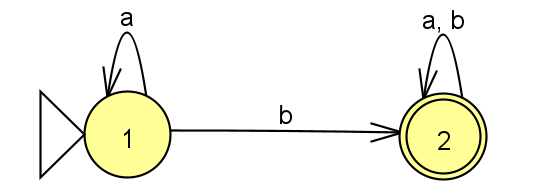
\includegraphics[scale=0.5]{../assets/dfa_regex_1.png}
\end{center}

\begin{enumerate}
    \item First, we need to convert this DFA to a GNFA. This would look like: 
    \begin{center}
        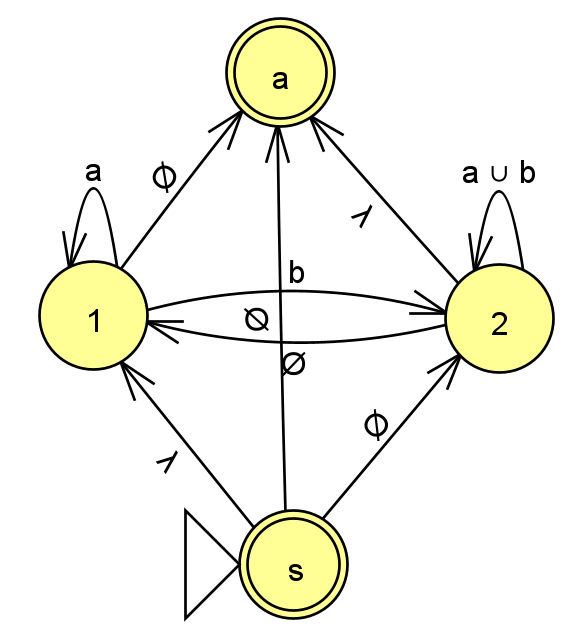
\includegraphics[scale=0.4]{../assets/dfa_regex_2.png}
    \end{center}
    Here, we've made a few changes. 
    \begin{itemize}
        \item First, we added two new states: $s$ for the new \emph{start} state and $a$ for the new \emph{accept} state. We have an arrow from $s$ to $1$ (the old start state) with $\epsilon$ as its label\footnote{The software used to create these state machines use $\lambda$ instead of $\epsilon$.}. We also have an arrow from $2$ (the old accept state) to $a$ with $\epsilon$ as its label. 
        \item Next, note that there was an arrow labeled $a, b$ at state $2$. We take the \emph{union} of these two labels to get $a \cup b$. Thus, state $2$ now has an arrow with $a \cup b$ instead of $a, b$. This is because the DFA's label represents two transitions, but a GNFA may only have a single transition going from a state to itself. 
        \item Finally, we add several arrows with the labels being $\emptyset$:
        \begin{itemize}
            \item $2$ to $1$ since every state needs to be able to transition to all non-start states. 
            \item $1$ to $a$ for the same reason as above. 
            \item $s$ to $2$ for the same reason as above. 
            \item $s$ to $a$ for the same reason as above. 
        \end{itemize}
    \end{itemize}

    \item Next, we pick one non-start/accept state as $q_{\text{rip}}$. We'll pick $2$ for our case, so let $2 = q_{\text{rip}}$. We're going to make use of the \code{CONVERT} algorithm. So, we pick $q_i = 1$ and $q_j = a$. Then: 
    \begin{itemize}
        \item $\delta(q_i, q_{\text{rip}}) = R_1 = b$
        \item $\delta(q_{\text{rip}}, q_{\text{rip}}) = R_2 = a \cup b$
        \item $\delta(q_{\text{rip}}, q_j) = R_3 = \epsilon$
        \item $\delta(q_i, q_j) = R_4 = \emptyset$
    \end{itemize}
    Therefore, $\delta'(q_i, q_j) = (b)(a \cup b)^* \epsilon \cup \emptyset$. This simplifies to $\delta'(q_i, q_j) = (b)(a \cup b)^*$. So, the corresponding new state diagram is: 
    \begin{center}
        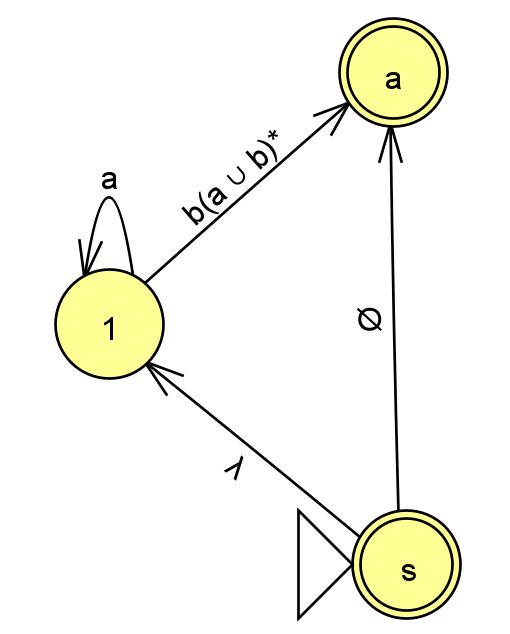
\includegraphics[scale=0.4]{../assets/dfa_regex_3.png}
    \end{center}

    \item We do this process again. We pick our one non-start/accept state as $q_{\text{rip}} = 1$. By our algorithm again, let $q_i = s$ and $q_j = a$. Then: 
    \begin{itemize}
        \item $\delta(q_i, q_{\text{rip}}) = R_1 = \epsilon$
        \item $\delta(q_{\text{rip}}, q_{\text{rip}}) = R_2 = a$
        \item $\delta(q_{\text{rip}}, q_j) = R_3 = b(a \cup b)^*$
        \item $\delta(q_i, q_j) = R_4 = \emptyset$
    \end{itemize}
    Therefore, $\delta'(q_i, q_j) = (\epsilon)(a)^* b(a \cup b)^* \cup \emptyset$. This can be simplified to $\delta'(q_i, q_j) = (a)^* b(a \cup b)^*$. So, the corresponding new state diagram is:
    \begin{center}
        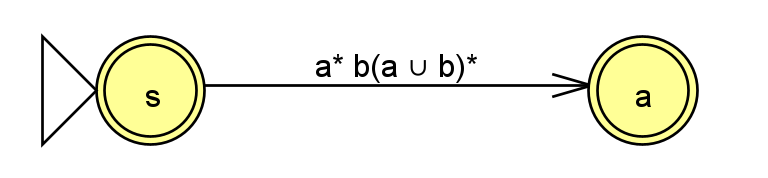
\includegraphics[scale=0.4]{../assets/dfa_regex_4.png}
    \end{center}
    Thus, the regular expression corresponding to the given DFA is $\boxed{(a)^* b(a \cup b)^*}$
\end{enumerate}

% Ø  ∪ λ


\subsection{Regular Expressions and Regularity of Language}
\begin{theorem}{}{}
    A language is regular if and only if some regular expression describes it. 
\end{theorem}

\begin{mdframed}[]
    \begin{proof}
        The proof is given by the two lemmas. 
    \end{proof}    
\end{mdframed}

\subsubsection{Regular Expression Implies Regularity}

\begin{lemma}{}{}
    If a language is described by a regular expression, then it is regular. 
\end{lemma}

\begin{mdframed}[]
    \begin{proof}
        Suppose we convert $R$ into an NFA $N$. We then need to consider six cases as defined by the formal definition of regular expression.
        \begin{enumerate}
            \item Let $R = a$ for some $a \in \Sigma$. Then, $L(R) = \{a\}$ and the following NFA recognizes $L(R)$:
            \begin{center}
                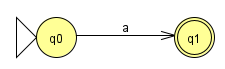
\includegraphics[scale=0.75]{../assets/nfa_regex_pf_1.png}
            \end{center}
            
            \item Let $R = \epsilon$. Then, $L(R) = \{\epsilon\}$ and the following NFA recognizes $L(R)$:
            \begin{center}
                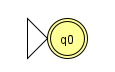
\includegraphics[scale=0.75]{../assets/nfa_regex_pf_2.png}
            \end{center}

            \item Let $R = \emptyset$. Then, $L(R) = \emptyset$ and the following NFA recognizes $L(R)$:
            \begin{center}
                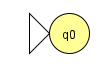
\includegraphics[scale=0.75]{../assets/nfa_regex_pf_3.png}
            \end{center}

            \item $R = R_1 \cup R_2$
            \item $R = R_1 \circ R_2$
            \item $R = R_{1}^*$
        \end{enumerate}
        Where the last three cases is given by a previous proof. 
    \end{proof}
\end{mdframed}

\subsubsection{Regularity Implies Regular Expression}

\begin{lemma}{}{}
    If a language is regular, then it is described by some regular expression.
\end{lemma}

\begin{mdframed}[]
    \begin{proof}
        If the language is regular, then it is accepted by a DFA. From the above, we've given a sketch of how to convert a DFA to a regular expression. 
    \end{proof}
\end{mdframed}

\end{document}